\section{Resultate}\label{resultate}
In diesem Abschnitt werden die Ergebnisse der Tests vorgestellt. Aufgrund dieser Resultate wurden die Lösungsansätze vom Abschnitt \ref{konzept} entwickelt. Für die PSNR-HVS-M Metrik existiert nicht immer ein Diagramm. Die Metrik wurde im Laufe der Arbeit entwickelt und wird ab Abschnitt \ref{resultate:loesung1:behandlung_ringing} ebenfalls gemessen.

\subsection{Lösungsansatz: Adaptives Subsampling} \label{resultate:loesung0}
Im Ist-Zustand führt der JHelioviewer nach der Dekompression ein adaptives Subsampling durch. Dieser Lösungsansatz führt das adaptive Subsampling vor der Datenübertragung durch und Kodiert die Daten mit Rar anstatt mit Gzip. Eine genauere Beschreibung des Ansatzes ist im Abschnitt \ref{konzept:loesung0} zu finden.
\begin{figure}[!htbp]
	\center
	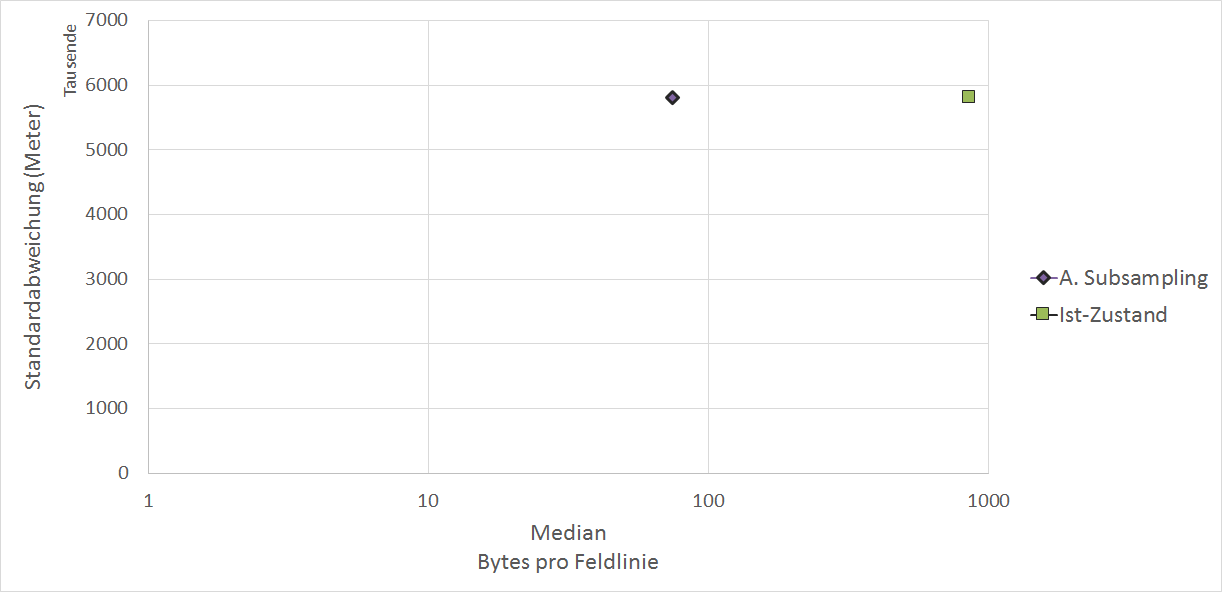
\includegraphics[width=1\textwidth,keepaspectratio]{./pictures/resultate/loesung0/loesung0_0.png}
	\caption{Vergleich des Lösungsansatzes: Adaptives Subsampling zur Ist-Kompression.}
	\label{resultate:loesung0:loesung0_0}
\end{figure}
Wie im Diagramm \ref{resultate:loesung0:loesung0_0} erkennbar ist, braucht dieser Lösungsansatz deutlich weniger Speicher als die Ist-Kompression. Das Adaptive Subsampling reduziert deutlich die Anzahl Punkte, während die Rar eine bessere Kompression erbringt. Dieser Ansatz kann die Daten um Faktor $11.6$ besser komprimieren.\\
\begin{figure}[!htbp]
	\center
	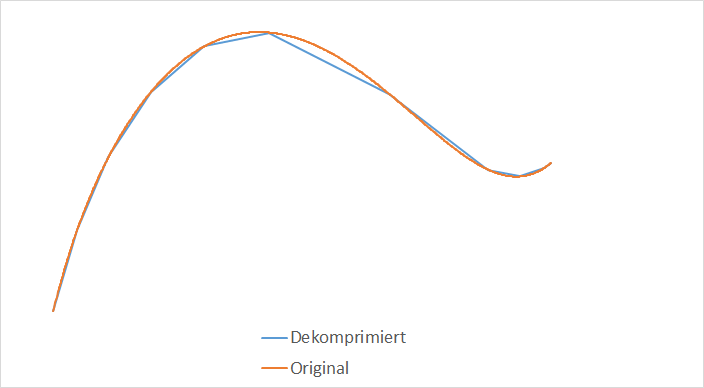
\includegraphics[width=1\textwidth,height=8cm,keepaspectratio]{./pictures/resultate/loesung0/loesung0_artefakte.png}
	\caption{Artefakte der Lösung 0}
	\label{resultate:loesung0:artefakte}
\end{figure}
Die Abbildung \ref{resultate:loesung0:artefakte} zeigt die Artefakte, die bei der Komprimierung der Lösung 0 entstehen. Es ist anzumerken, dass der Ist-Zustand die selben Artefakte aufweist.
\pagebreak

\subsection{Lösungansatz: Diskrete Kosinus Transformation}
In diesem Abschnitt wird der Lösungsansatz mittels Diskreter Kosinus Transformation behandelt. Es wurden verschiedene Transformationen getestet, welche eine Approximation mittels Kosinus Funktionen vereinfachen könnten.\\
Um die Feldlinien optimal mit der DCT zu approximieren, müssen Ringing Artefakte, behandelt werden. Das Auftreten der Artefakte wird im Abschnitt \ref{resultate:loesung1:ringing} und die Behandlung im Abschnitt \ref{resultate:loesung1:behandlung_ringing} besprochen .\\
[\baselineskip]
Für alle Tests wurde eine lineare Quantisierung verwendet. Jeder DCT Koeffizient wird durch einen Faktor geteilt, der sich stetig ehöht. Zum Beispiel wird der erste Koeffizient durch zwei geteilt, der zweite durch Vier, der Dritte durch Sechse etc.  Die Kompressionsrate kann durch einen höheren oder tieferen Faktor gesteuert werden. Diese Quantifizierung ist nicht das Optimum. Eine bessere Quantifizierung wird für die beste Variante ausgearbeitet. Wie die beste Variante im Detail umgesetzt wurde, wird im Abschnitt \ref{konzept:loesung0:kodierung} behandelt. 

\subsubsection{Variante: DCT}\label{resultate:dct}
Diese Variante verwendet einzig die Diskrete Kosinus Transformation und der linearen Quantisierung.
\begin{figure}[!htbp]
	\center
	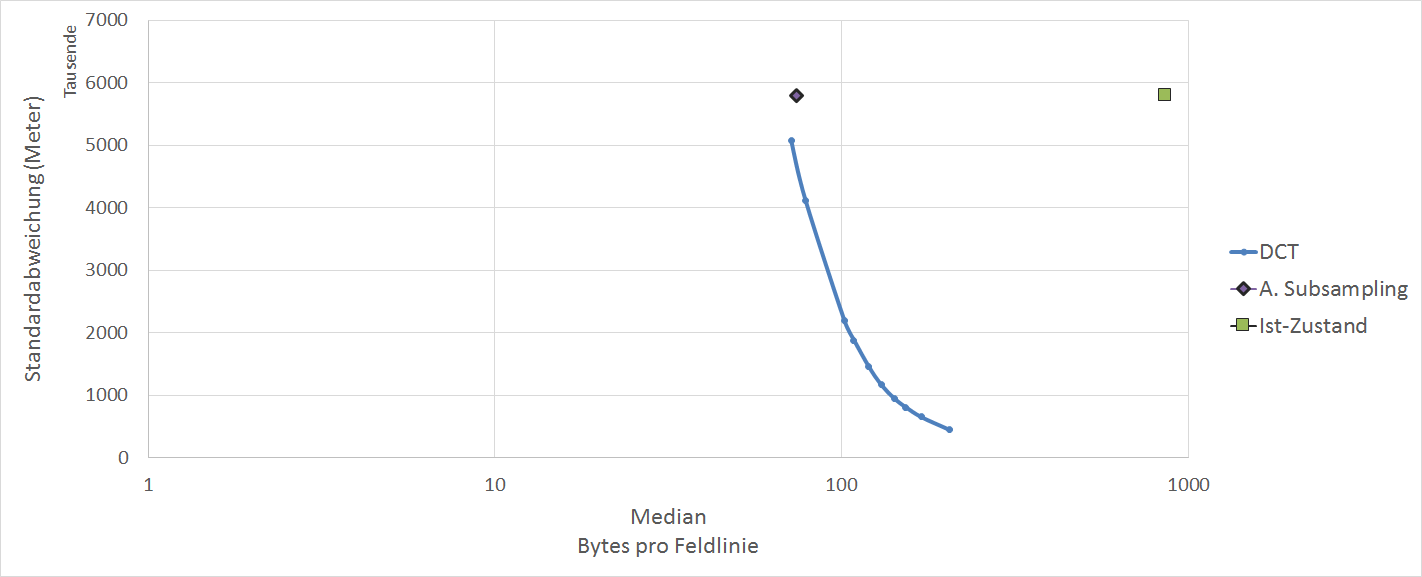
\includegraphics[width=1\textwidth,keepaspectratio]{./pictures/resultate/loesung1/loesung1-0/loesung1_0.png}
	\caption{Vergleich der DCT Kompression mit der Lösung0}
	\label{resultate:loesung1:dct:resultate}
\end{figure}
Die Abbildung \ref{resultate:loesung1:dct:resultate} zeigt den Vergleich der DCT Kompression mit dem Lösungsansatz des Adaptiven Subsamplings (siehe \ref{resultate:loesung0}). Es ist deutlich zu erkennen, dass die Standardabweichung schnell steigt bei leicht sinkender Grösse. Der Grund dafür kann im Diagramm der Abbildung \ref{resultate:loesung1:dct:artefakte} entnommen werden. 
\begin{figure}[!htbp]
	\center
	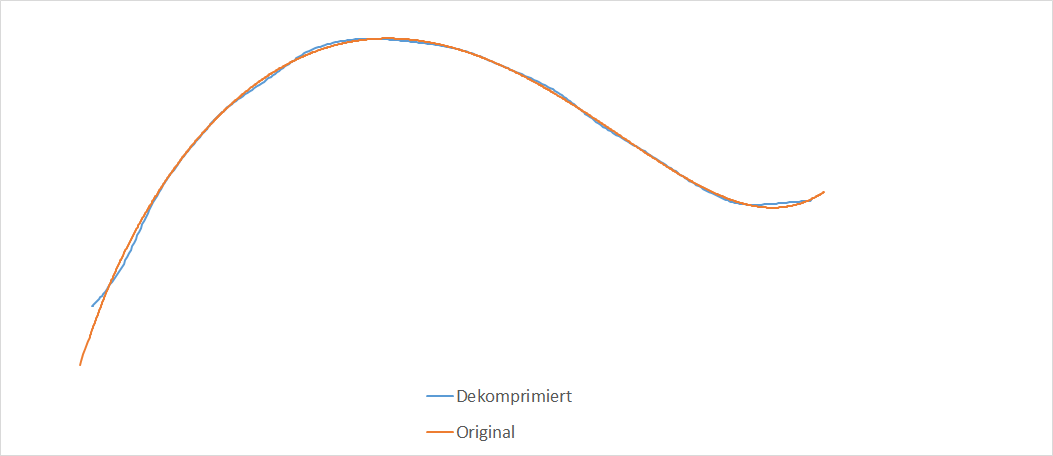
\includegraphics[width=0.8\textwidth,height=8cm,keepaspectratio]{./pictures/resultate/loesung1/loesung1-0/loesung1_0_artefakte.png}
	\caption{Artefakte der DCT Dekompression anhand Beispieldaten}
	\label{resultate:loesung1:dct:artefakte}
\end{figure}
Un den meisten Fällen kann die DCT die Feldlinie gut approximieren. Bei dieser Feldlinie wird der Anfang der Kurve nicht richtig dargestellt. Das ist ein typisches Problem der DCT. Die Diskrete Kosinus Transformation nimmt an, dass das Signal sich periodisch wiederholt. Die implemementierte Transformation (siehe Abschnitt \ref{konzept:loesung1:kosinus}) nimmt an, dass am Anfang und am Ende das Signal in umgekehrter Reihenfolge wiederholt. Bei den Feldlinien kann das zu einer Diskontinuität im Signal führen, welches hochfrequente Kosinus Anteile. Wenn die Quantisierung Hochfrequente Schwingungen verschluckt, entstehen die Artefakte der Abbildung \ref{resultate:loesung1:dct:artefakte}.\\
Eine Möglichkeit ist die Feldlinie um Punkte zu erweitern. Wenn die Feldlinie am Anfang und am Ende abflacht, sollte die resultierende Transformation weniger hochfrequente Schwingungen enthalten. Diese Variante wird im Abschnitt \ref{resultate:loesung1:dct:randbeh+byte} behandelt und führt zu einer deutlich besseren Approximation. Durch eine andere Darstellung der Daten kann das Problem ebenfalls gelöst werden.

\subsubsection{Variante: Ableitung+DCT}\label{resultate:dct:ableitung_dct}
Vor der DCT werden die Feldlinien abgeleitet. Mit der Ableitung soll das Randproblem dargestellt in \ref{resultate:loesung1:dct:artefakte} gelöst werden. Der Nachteil ist, dass Ungenauigkeiten sich durch die Kurve durchziehen und summieren. Am Ende kann die Approximation ungenauer sen, wie am Anfang der Feldlinie.\\
\begin{figure}[!htbp]
	\center
	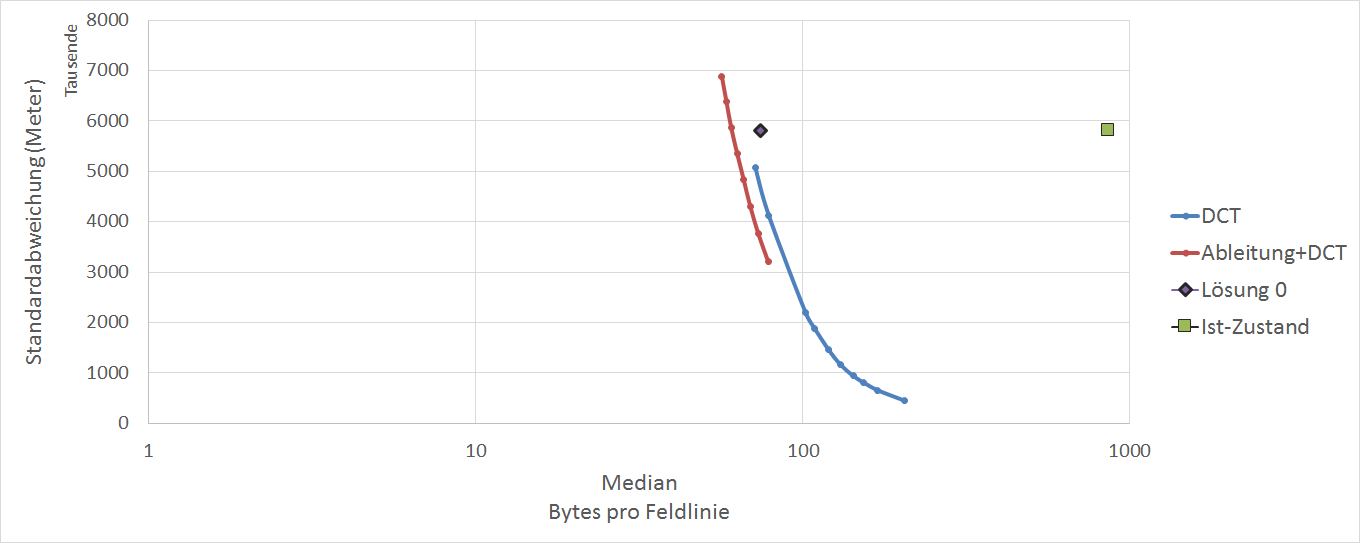
\includegraphics[width=1\textwidth,keepaspectratio]{./pictures/resultate/loesung1/loesung1-1/loesung1_1.png}
	\caption{Vergleich der DCT Kompression der Ableitung mit der DCT Kompression}
	\label{resultate:loesung1:dct_ableitung:resultate}
\end{figure}
Das Diagramm der Abbildung \ref{resultate:loesung1:dct_ableitung:resultate} zeigt, dass die abgeleiteten Feldlinien besser approximiert werden können und erreichen dadurch eine Kompressionsrate von $14.3$ mit einer vergleichbaren Genauigkeit. Das Randproblem wurde ebenfalls verbessert. Eine Darstellung der Artefakte ist im Diagramm der Abbildung\ref{resultate:loesung1:dct:byte:artefakte} zu finden.\\
\begin{figure}[!htbp]
	\center
	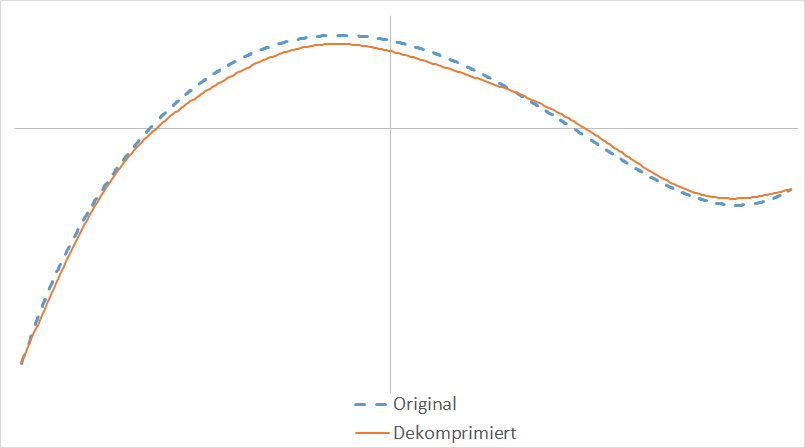
\includegraphics[width=0.8\textwidth,height=8cm,keepaspectratio]{./pictures/resultate/loesung1/loesung1-6/artefakte.png}
	\caption{Artefakte der DCT Kompression der Ableitung}
	\label{resultate:loesung1:dct:byte:artefakte}
\end{figure} 
Es ist deutlich zu sehen, dass die Kurve durch die Quantisierung gedämpft wird. das Maximum der Kurve ist tiefer, sowie das lokale Minima der letzten Halbwelle höher. Der Vorteil dieser Variante ist, dass die resultierende Feldline sehr glatt verläuft. Ohne die Originalkurve währen die Artefakte nicht zu identifizieren.

\subsubsection{Variante: PCA+Ableitung+DCT}
Die Feldlinien liegen meist auf einer Ebene im dreidimensionalen Raum. Wenn die X,Y und Z Kanäle Kosinus-Transformiert werden, ist die Information etwa gleichmässig auf den Kanälen verteilt. Eine Linie könnte sich durch weniger Kosinus-Funktionen approximieren lassen, wenn die Linie zuerst in ein lokales Koordinatensystem transformiert wird.\\
Die Principal Component Analysis (PCA)\cite{abdi2010principal} ist ein Verfahren aus der Statistik, welches Daten in ein neues koordinatensystem Transformiert. Dabei werden die Achsen so gelegt, dass die Daten entlang der ersten Achse die grösste Varianz aufweisen, entlang der zweiten Achse, welche orthogonal zur ersten liegt, die zweithöchste Varianz etc. Wenn das Vefahren auf die Feldlinien angewandt wird, werden die Feldlinien in ein lokales System transformiert indem der Z-Kanal 0 ist, wenn die Feldlinie in einer Ebene liegt..\\
Um die PCA wieder rückgängig zu machen, müssen pro Feldlinie sechs Parameter für die neuen Koordinatenachsen und 3 Parameter für die Verschiebung abgespeichert werden.
\begin{figure}[!htbp]
	\center
	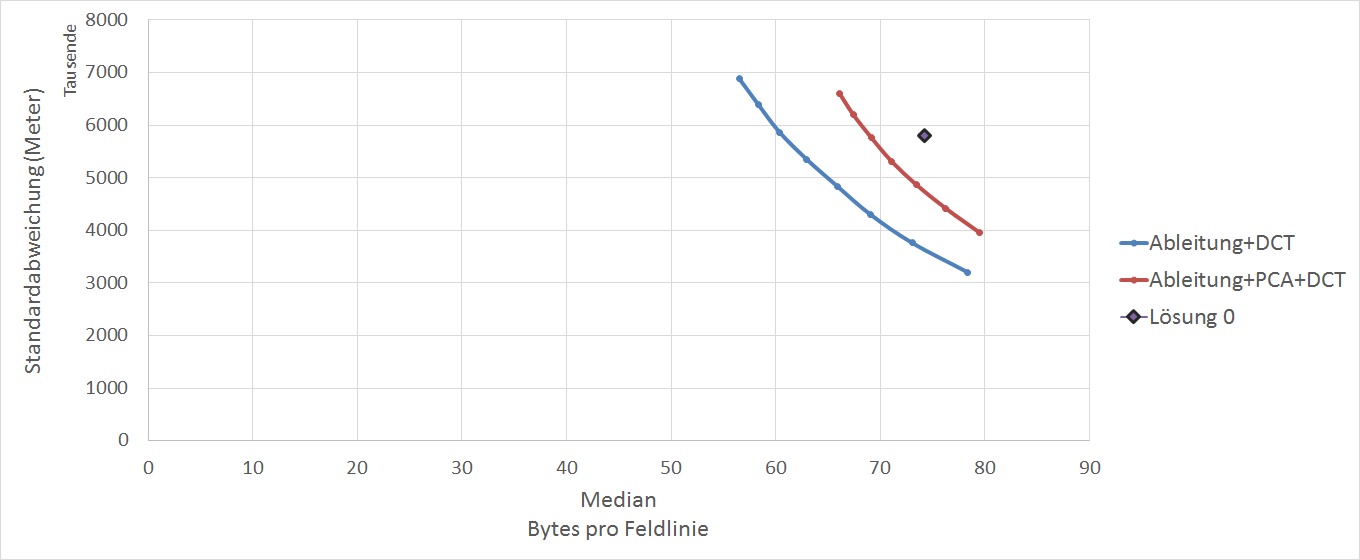
\includegraphics[width=1\textwidth,keepaspectratio]{./pictures/resultate/loesung1/loesung1-4/loesung1_4.png}
	\caption{Vergleich der PCA DCT Kompression der Ableitung mit der DCT Kompression der Ableitung}
	\label{resultate:loesung1:dct:pca}
\end{figure}
Die PCA scheint die Kompression nicht verbessern zu können. Der Grund ist, dass die Variante ohne PCA zwischen 5 und 20 Kosinus-Funktionen braucht, um einen Kanal einer Feldlinie zu approximieren. Durch die PCA können 2-5 Parameter gespart werden, jedoch verbrauchen die zusätzlichen Koordinatenachsen und Verschiebungen mehr Speicher, als die Transformation gewinnt.

\subsubsection{Variante: Ableitung+DCT+Byte Kodierung} \label{resultate:loesung1:ableitung_dct_kodierung}
Ein Kanal einer Feldlinie kann mit 5-20 DCT-Koeffizienten ausreichend approximiert werden. Die quantisieren Koeffizienten kommen meistens zwischen -50 und +50 zu liegen. 8 Bit Genauigkeit reichen im Allgemeinen aus, um einen quantisierten Koeffizienten abzuspeichern. Um die Kompressionsrate zu verbessern, werden zwei Byte-Kodierungen eingeführt: die Längenkodierung und die Byte-Kodierung (beschrieben im Abschnitt \ref{konzept:loesung1:kodierung}).\\
\begin{figure}[!htbp]
	\center
	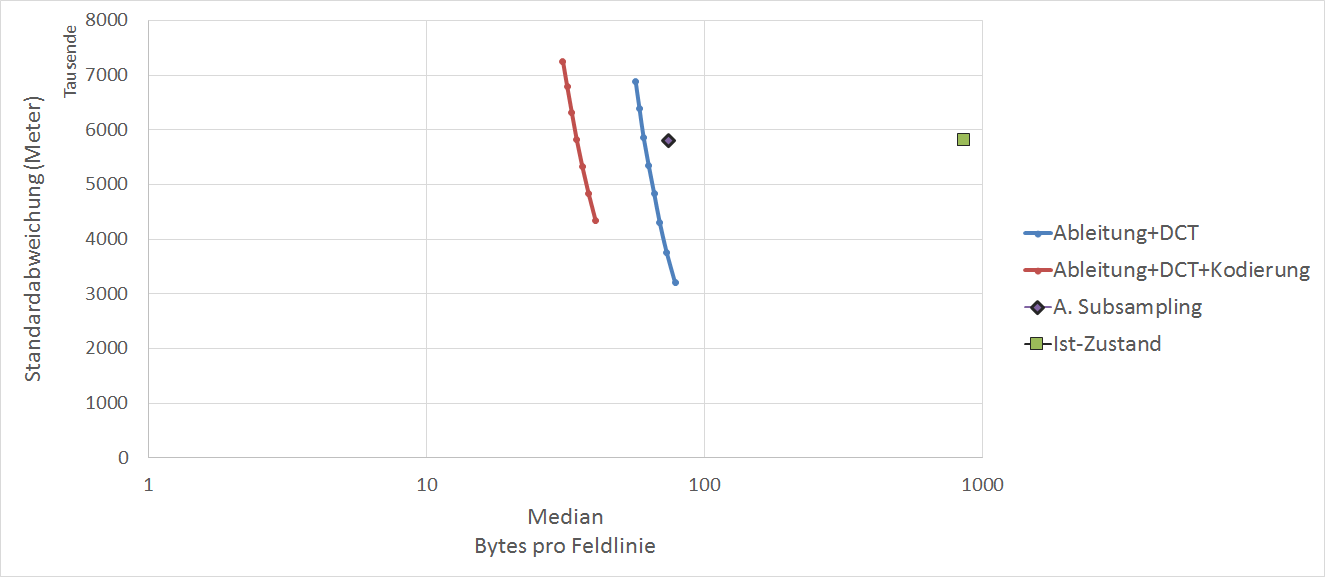
\includegraphics[width=1\textwidth,keepaspectratio]{./pictures/resultate/loesung1/loesung1-6/loesung1_6.png}
	\caption{Vergleich der Kompression mit und ohne Byte-Kodierung}
	\label{resultate:loesung1:dct:kodierung}
\end{figure}
Das Diagramm der Abbildung \ref{resultate:loesung1:dct:kodierung} zeigt den Einfluss der Byte-Kodierung auf die Kompressionsrate. Es bewirkt eine deutliche Verbesserung, ohne die Qualität der Kompression negativ zu beeinflussen. Bei einer Vergleichbaren Genauigkeit wie die Ist-Lösung weist diese Variante eine Kompressionsrate von $24.5$ auf.

\subsubsection{Variante: Randbehandlung+DCT+Byte Kodierung} \label{resultate:loesung1:dct:randbeh+byte}
Wenn  die Artefakte \ref{resultate:loesung1:dct:byte:artefakte} und \ref{resultate:loesung0:artefakte} vergleicht, fällt auf, dass die Variante \ref{resultate:dct} die Feldlinie genauer approximiert, falls die Ränder der Feldlinie besser dargestellt werden könnte. Wenn die Feldlinie an den Rändern mit Punkten erweitert wird, welche die Transformation vereinfachen, könnte eine bessere Kompression erreicht werden.\\
Jeder Kanal einer Feldlinie wird so erweitert, dass der Anfang und das Ende abflacht. Die Byte-Kodierung wurde aus der vorhergehenden Variante übernommen.
\begin{figure}[!htbp]
	\center	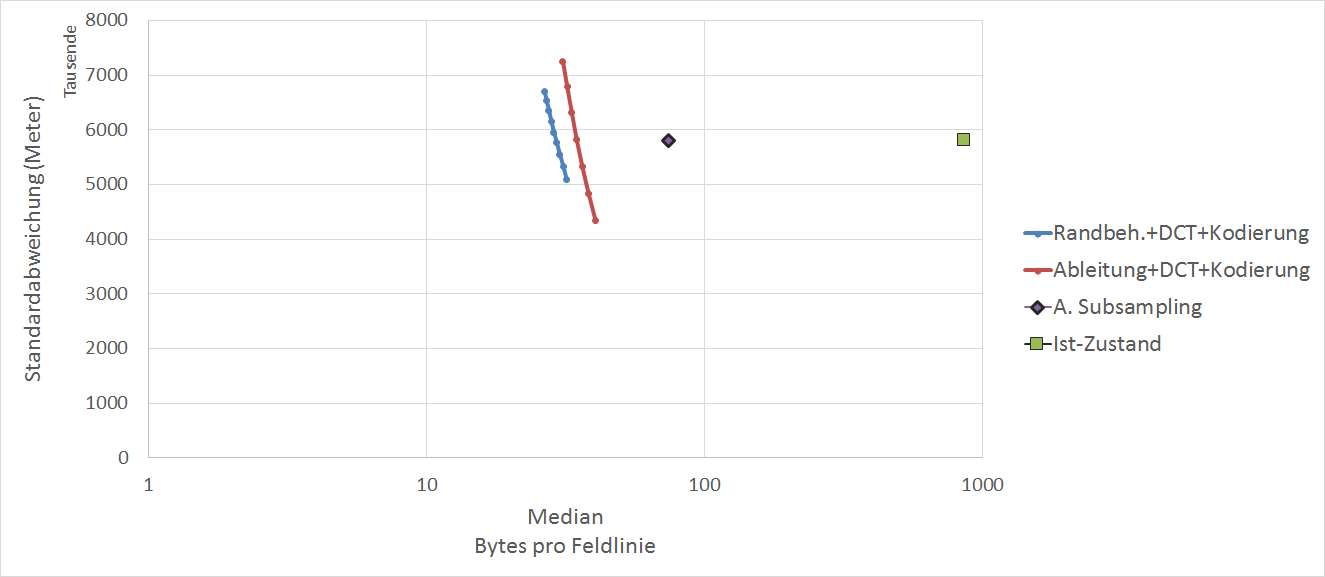
\includegraphics[width=1\textwidth,keepaspectratio]{./pictures/resultate/loesung1/loesung1-7/loesung1_7.png}
	\caption{Vergleich des Einflusses der Randbehandlung}
	\label{resultate:loesung1:dct:randbehandlung}
\end{figure}
Das Diagramm der Abbildung \ref{resultate:loesung1:dct:randbehandlung} zeigt den Vergleich der Variante mit Randbehandlung und der Variante der abgeleiteten Feldlinie (beschrieben im Abschnitt \ref{resultate:loesung1:ableitung_dct_kodierung}. Es ist zu erkennen, dass dank der Randbehandlung die Feldlinien mit weniger Bytes ähnlich genau approximiert werden können.\\
Diese Variante führt aber Artefakte ein, welche die Standardabweichung nicht erkennen kann. Im Folgenden Abschnitt \ref{resultate:loesung1:ringing} werden diese besprochen.

\subsubsection{Ringing Artefakte}\label{resultate:loesung1:ringing}
Obwhol die Variante \ref{resultate:loesung1:dct:randbeh+byte } eine vergleichbare Genauigkeit aufweist, wie die Ist-Lösung, sind auf der JHelioviewer Visualisierung deutliche Artefakte zu sehen. Die Abbildung \ref{resultate:loesung1:dct:randbehandlung:jvhartefakte} vergleicht die originalen mit dekomprimierten Feldlinien. Die Artefakte zeigen sich als Oszillationen.
\begin{figure}[!htbp]
	\center
	\frame{
	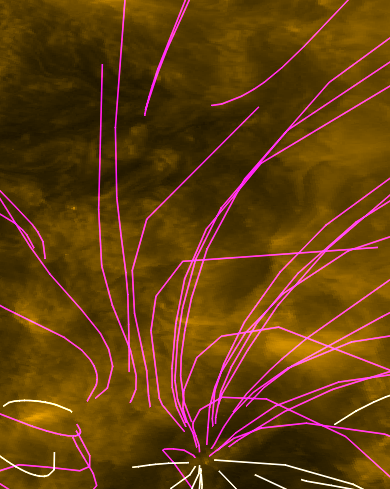
\includegraphics[width=0.8\textwidth,height=6cm,keepaspectratio]{./pictures/resultate/loesung1/ringing/actual.png}}
		\frame{
	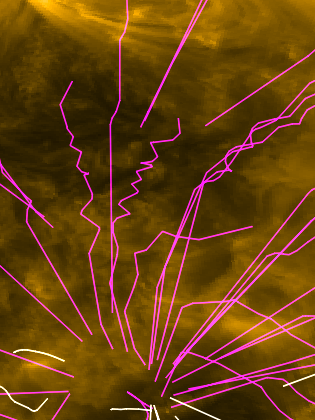
\includegraphics[width=0.8\textwidth,height=6cm,keepaspectratio]{./pictures/resultate/loesung1/ringing/sol7.png}}
	\caption{Artefakte der Kompression, links sind die originalen Feldlinien, rechts die Dekomprimierten.}
	\label{resultate:loesung1:dct:randbehandlung:jvhartefakte}
\end{figure} 
In diesem Fall scheint die Standardabweichung als Fehlermass zu versagen: Da die Oszillationen nahe an der originalen Feldlinie liegen, bleiben die Abstände klein. Jedoch sind die Artefakte für das menschliche Auge inakzeptabel.\\
Interessant ist, dass die die Variante der Ableitung (Abschnitt \ref{resultate:loesung1:ableitung_dct_kodierung}) ähnliche Artefakte aufweist. Im Diagramm der Abbildung \ref{resultate:loesung1:dct:byte:artefakte}, welches die Artefakte anhand einer Beispiellinie zeigt, sind keine Oszillationen zu entdecken. In der JHelioviewer Visualisierung jedoch, sind auch bei dieser Variante deutliche Oszillationen zu erkennen. Die Abbildung \ref{resultate:loesung1:dct:randbehandlung:jvhartefakte_loesung6} zeigt die Artefakte. Es ist anzumerken, dass die Artefakte weniger ausgeprägt sind, aber dennoch störend für das menschliche Auge.\\
\begin{figure}[!htbp]
	\center
	\frame{
	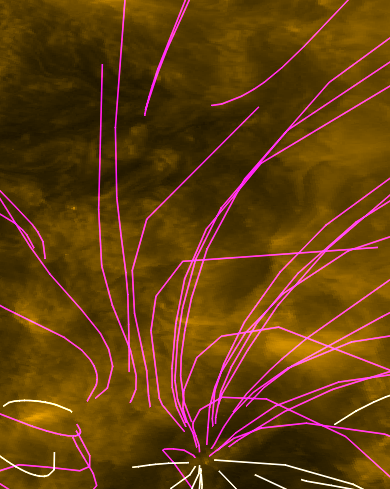
\includegraphics[width=0.8\textwidth,height=6cm,keepaspectratio]{./pictures/resultate/loesung1/ringing/actual.png}}
		\frame{
	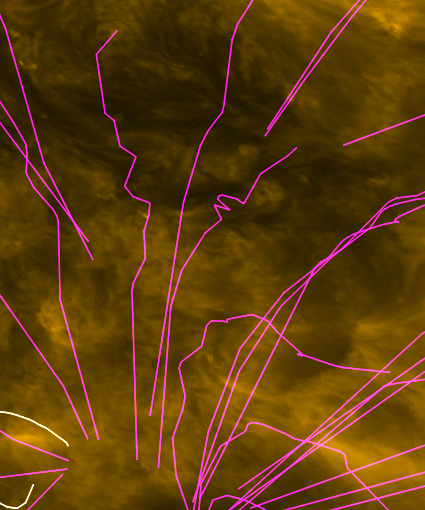
\includegraphics[width=0.8\textwidth,height=6cm,keepaspectratio]{./pictures/resultate/loesung1/ringing/sol6.png}}
	\caption{Artefakte der Kompression, links sind die originalen Feldlinien, rechts die Dekomprimierten der Variante \ref{resultate:loesung1:ableitung_dct_kodierung}.}
	\label{resultate:loesung1:dct:randbehandlung:jvhartefakte_loesung6}
\end{figure}
Die oszillierenden Artefakte sind typisch für eine DCT-Kompression und sind im Allgemeinen als Ringing Artefakte \cite{wiki:ringing:artefacts} bekannt: Abrupte Steigungen im Inputsignal werden in der DCT durch hochfrequente Anteile dargestellt. Durch die Quantisierung der hochfrequenten Anteile werden oszillierende Artefakte eingefügt. Die Ringing Artefakte typische Kompressionsartefakte von DCT-basierten Verfahren wie JPEG/JFIF oder MP3.\\
Die Feldlinien, welche am stärksten von den Artefakten betroffen sind, sind die ''Weltall zur Sonne'' oder ''Sonne ins Weltall'' Feldlinien. Sie verhalten sich nicht wie harmonische Halbwellen sondern steigen oft monoton, mit teils abrupten Richtungswechseln in der Nähe der Sonnenoberfläche. Die Abbildung \ref{resultate:loesung1:dct:randbehandlung:harte_richtungswechsel} zeigt ein Beispiel solcher Feldlinien. Die abrupten Wechsel führen zu abrupten Steigungen in den einzelnen Kanälen.
\begin{figure}[!htbp]
\center
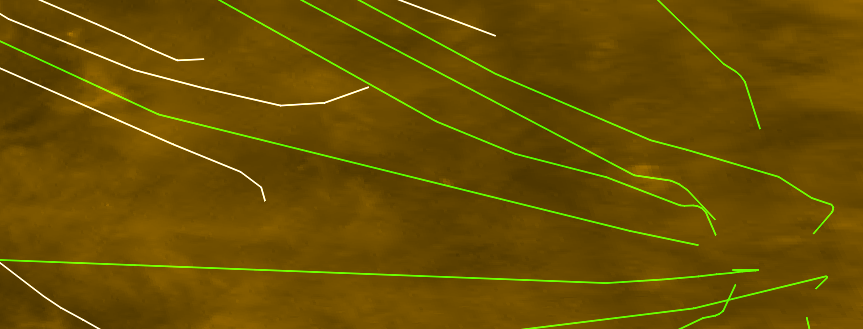
\includegraphics[width=0.4\textwidth,height=6cm,keepaspectratio]{./pictures/resultate/loesung1/ringing/haar-like.png}
	\caption{Abrupte Steigungen bei Feldlinien, welche von der Sonne ins Weltall führen.}
	\label{resultate:loesung1:dct:randbehandlung:harte_richtungswechsel}
\end{figure}

\subsubsection{Behandlung der Ringing Artefakte} \label{resultate:loesung1:behandlung_ringing}
Um eine optimale Kompression der Feldlinien zu erreichen, müssen die Ringing Artefakte behandelt werden. Abschnitt \ref{resultate:loesung1:ringing} wurde erwähnt, dass nicht alle Varianten gleich starke Artefakte verursachen. Es wurde ebenfalls besprochen, dass die Feldlinien, welche von der Sonnenoberfläche zur Oberfläche führen, kaum von den Artefakten betroffen sind. In diesem Abschnitt wird deshalb erforscht, welche Variante die ''Sonne zu Sonne'' und welche die ''Weltall zur Sonne'' oder ''Sonne ins Weltall'' Feldlinien optimal approximieren kann. Für die Messung der Artefakte wird die PSNR-HVS-M Metrik aus Abschnitt \ref{testsetup:psnr} verwendet.\\
Für den Test werden insgesamt vier Varianten verglichen. Die Varianten \ref{resultate:loesung1:ableitung_dct_kodierung} und und \ref{resultate:loesung1:dct:randbeh+byte} jeweils mit und ohne PCA Transformation. Die Transformation wird hier nochmals geprüft. Die Transformation könnte die Rining Artefakte jeweils auf einen Kanal beschränken.\\
\begin{figure}[!htbp]
	\center	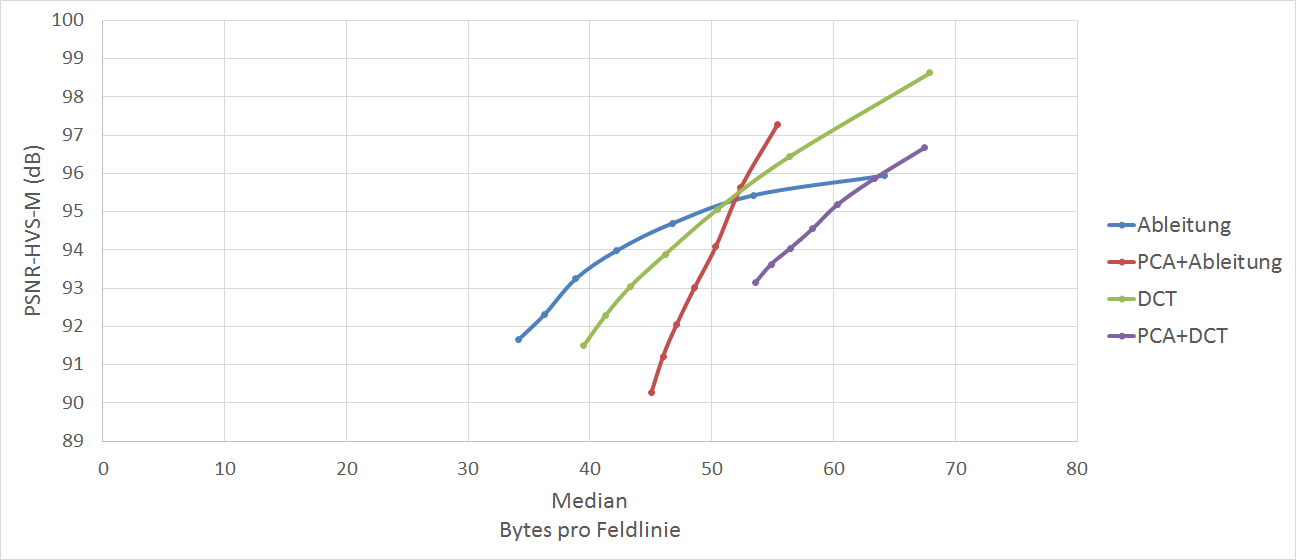
\includegraphics[width=1\textwidth,keepaspectratio]{./pictures/resultate/loesung1/ringing/sts.png}
	\caption{Approximation der Feldlinien ''Sonnenoberfläche zu Sonnenoberfläche''. Je höher die PSNR-HVS-M, desto besser ist die Approximation. }	\label{resultate:loesung1:dct:behandlung_ringing:sts}
\end{figure} 
\begin{figure}[!htbp]
	\center
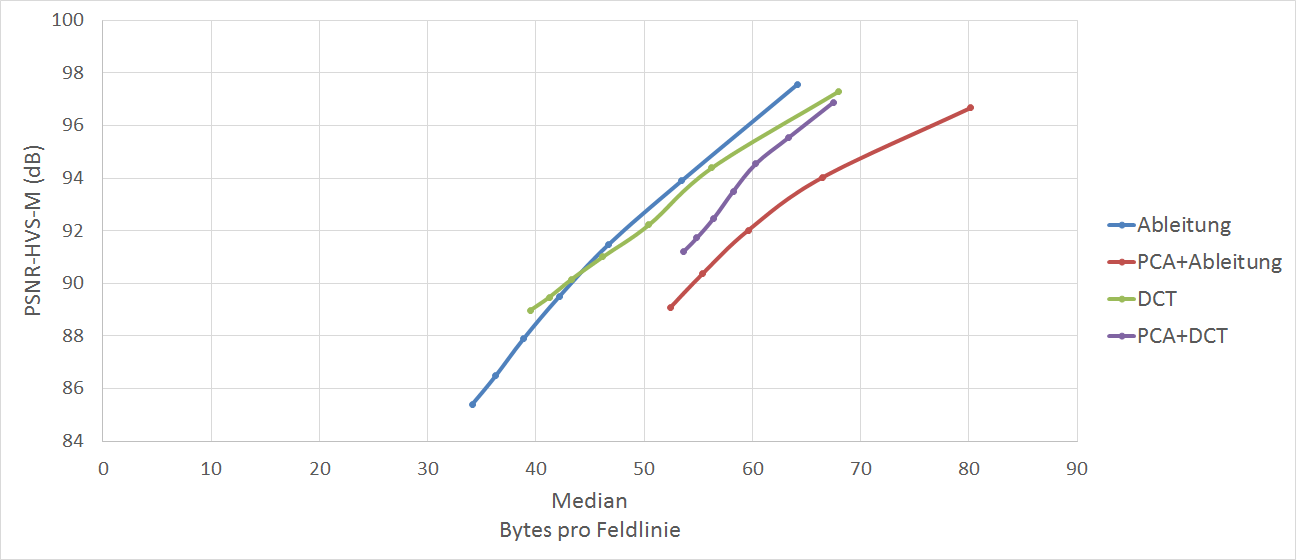
\includegraphics[width=1\textwidth,keepaspectratio]{./pictures/resultate/loesung1/ringing/nosts.png}
	\caption{Approximation der der Feldlinien ''Sonnenoberfläche ins Weltall'' oder ''Weltall zur Sonnenoberfläche''. Je höher die PSNR-HVS-M, desto besser ist die Approximation.}	\label{resultate:loesung1:dct:behandlung_ringing:nosts}
\end{figure}
Das Diagramm der Abbildung \ref{resultate:loesung1:dct:behandlung_ringing:sts} zeigt, wie gut die Varianten die Feldlinien approximieren können, welche von der Sonnenoberfläche zur Sonnenoberfläche führen. Es ist anzumerken, dass ein PSNR-HVS-M Wert von etwa $95 dB$ bedeutet, dass die Feldlinien kaum sichtbare Artefakte enthalten. Je höher der PSNR-HVS-M Wert, desto genauer ist die Approximation. Interessant ist, dass drei Varianten ähnlich viel Speicherplatz benötigen, für eine beinahe artefaktfreie Approximation. Bei stärkerer Quantisierung treten beiden abgeleiteten Feldlinien deutlich weniger Artefakte auf. Dies deckt sich mit den Beobachtung aus dem Abschnitt \ref{resultate:loesung1:ringing}.\\
Ebenfalls interessant ist die Variante der PCA Transformation zusammen mit der Ableitung: Diese benötigt für eine beinahe artefaktfreie Approximation am wenigsten Speicherplatz, führt aber bei stärkerer Quantisierung viele Artefakte ein.

Das Diagramm der Abbildung  \ref{resultate:loesung1:dct:behandlung_ringing:nosts} zeigt, wie gut die Varianten die die andern Typen von Feldlinien approximieren können. Hier ist zu sehen, dass die abgeleiteten Feldlinien weniger Artefakte hinzufügen, jedoch weniger deutlich als in der Abbildung \ref{resultate:loesung1:dct:behandlung_ringing:sts}. Interessant ist, dass die PCA keinen messbaren Vorteil erbrachte. Die zusätzlichen Parameter, die für die Umkehrung der PCA abgespeichert werden, verbrauchen mehr Speicherplatz als man durch die Transformation gewinnt.\\
Die DCT Variante aus Abschnitt \ref{resultate:loesung1:dct:randbeh+byte} fällt ab einer PSNR-HVS-M von $90 dB$ weniger schnell ab, als die abgeleiteten Feldlinien. Bei diesem PSNR-HVS-M Wert sind aber die Artefakte bereits zu deutlich und nicht mehr akzeptabel. Aufgrund dieser Daten wurde die Variante unter Abschnitt \ref{resultate:loesung1:ableitung_dct_kodierung} ausgewählt. 

\subsubsection{Abschliessende Variante}
Für den abschliessenden Test wurde die Variante unter Abschnitt \ref{resultate:loesung1:ableitung_dct_kodierung} ausgewählt. Diese verursacht weniger starke Ringing Artefakte als die anderen Varianten. Dies liegt an der Artefaktdämpfenden Eigenschaft der Ableitung und an der auf die auf den Typ angepasste Quantisierung.
\begin{figure}[!htbp]
	\center	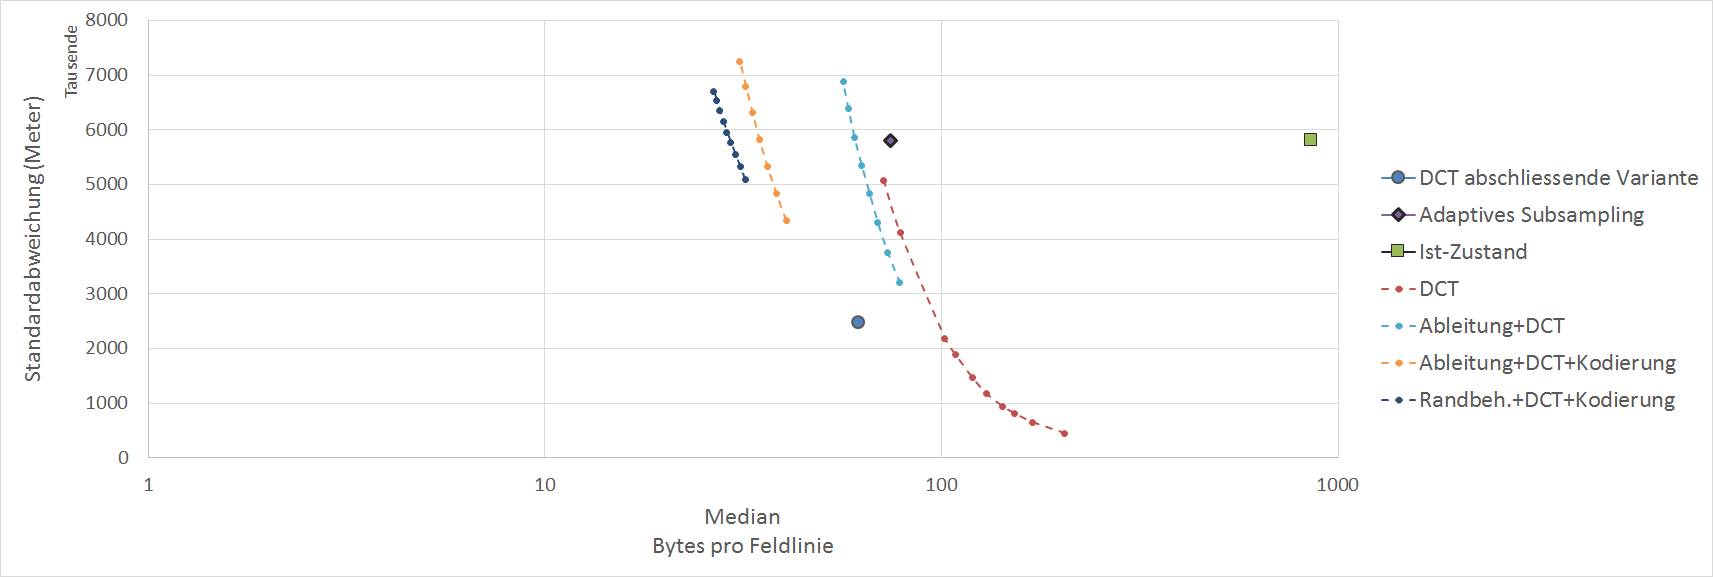
\includegraphics[width=1\textwidth,keepaspectratio]{./pictures/resultate/loesung1/loesung1-12/resultate.png}
	\caption{Standardabweichung der abschliessenden DCT Variante.}	\label{resultate:loesung1:dct:abschliessend:standardabweichung}
\end{figure} 
Das Diagramm der Abbildung \ref{resultate:loesung1:dct:abschliessend:standardabweichung} zeigt die Standardabweichung der abschliessenden DCT Variante. Zu einer besseren Kompression kann sie deutlich genauer Punkte ablegen und erreicht eine Kompressionsrate von $14.1$. Die Artefakte sind mit einer PSNR-HVS-M von $94.0$ ebenfalls in Grenzen gehalten. Jedoch sind wegen dem Zoom-Feature des JHelioviewers immer noch Oszillationen zu erkennen. Das Linke Bild der Abbildung \ref{resultate:loesung1:dct:final:artefakte} zeigt die Artefakte der Dekompression. Die Artefakte sind aus der Simulation, welche diese Variante am schlechtesten approximieren konnte. Es ist ebenfalls anzumerken, dass die Artefakte bei weniger hohen Zoomstufen nicht mehr zu erkennen sind.
\begin{figure}[!htbp]
	\center
	\frame{
	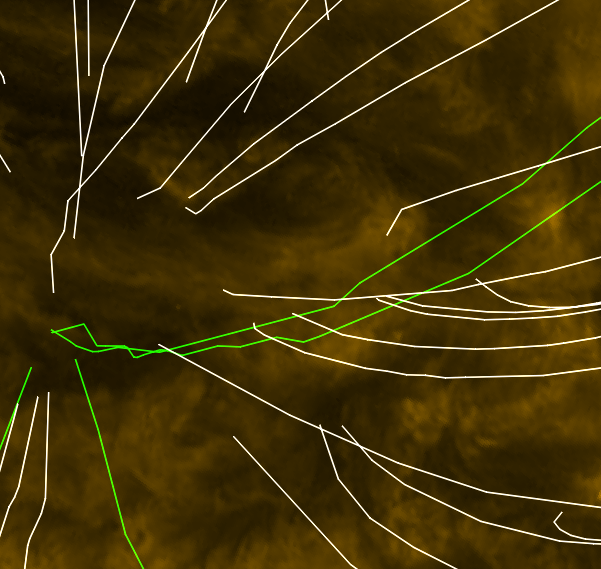
\includegraphics[width=0.8\textwidth,height=5cm,keepaspectratio]{./pictures/resultate/loesung1/loesung1-12/without_average_line.png}}
		\frame{
	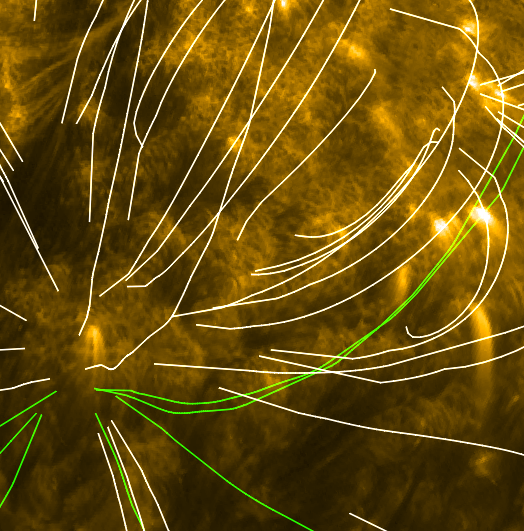
\includegraphics[width=0.8\textwidth,height=5cm,keepaspectratio]{./pictures/resultate/loesung1/loesung1-12/with_average_line.png}}
	\caption{Artefakte der abschliessenden Variante. Links ohne Glättung, rechts mit Glättung}
	\label{resultate:loesung1:dct:final:artefakte}
\end{figure}
Die Verbesserung in der Genauigkeit wurde erreicht, indem die Feldlinientypen unterschiedlich quantisiert wurden. Die ''Sonne zu Sonne'' können mit wenigeren Koeffizienten approximiert werden als die anderen Typen. Würde die Simulation nur aus diesen Feldlinien bestehen, könnte eine Kompressionsrate von $18-20$ erreicht werden zu einer ähnlichen Genauigkeit. Die Schwierigkeit liegt darin die anderen Feldlinien mit möglichst wenigen Artefakten zu approximieren. Eine Kompression mit der Diskreten Kosinus Transformation wird ab einer gewissen Zoom-Stufe immer Artefakte mit sich bringen, welche das menschliche Auge erkennen kann.\\
Der JHelioviewer kann die Artefakte verschleiern mit einer Kurvenglättung: Die komprimierten Daten enthalten mehr Punkte, als der JHelioviewer darstellen könnte. Die zusätzlichen Punkte können für die Glättung der Feldlinie verwendet werden. Den Effekt der Glättung ist in der Abbildung \ref{resultate:loesung1:dct:final:artefakte} verdeutlicht. Dadurch können die Artefakte auch bei höheren Zoomstufen verschleiert werden. Im Abschnitt \ref{konzept:loesung1} wurde erwähnt, dass reduktion von Ringing Artefakte ein aktives Forschungsfeld der Bildverarbeitung ist. Es existieren Post-Processing Filter, welche Ringing Artefakte vermindern. Eine Möglichkeit die Kompression zu verbessern ist es, einen Post-Processing Filter für wissenschaftliche Daten zu entwickeln.
\pagebreak
\subsection{Lösungsansatz: Prediktive Kodierung}
Wie daten verloren gehen, warum 

\subsubsection{Variante: einfaches Subsampling}
PCA + PCA erlaubt es, 16 Bit zu speichern.
Für den Test dieser Variante wurde den Einfluss von vier Prediktoren überprüft:
\begin{itemize}
\item Konstanter Prediktor: Nimmt an, dass der nächste Wert im Signal gleich dem letzten Wert ist.
\item Linearer Prediktor: Nimmt an, dass der nächste Wert auf der Gerade z
\item Linearer Prediktor mit Moving Average: 
\item Adaptiver Linearer Prediktor mit Moving Average:
\end{itemize}
Wer die beste vorhersage machen kann
\begin{figure}[!htbp]
	\center
	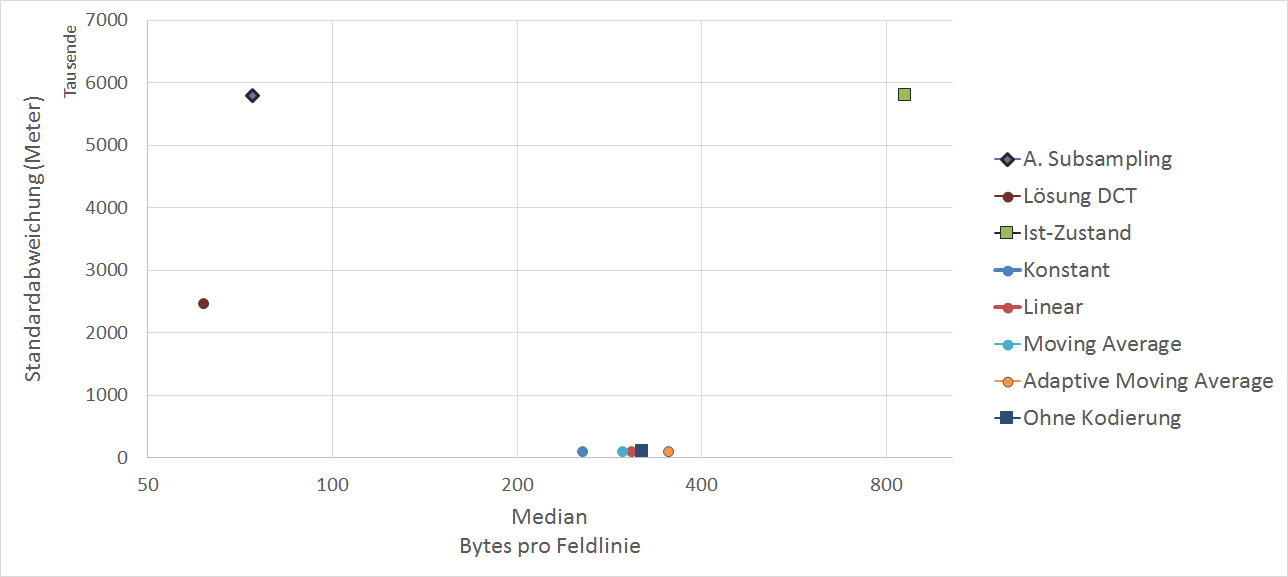
\includegraphics[width=1\textwidth,keepaspectratio]{./pictures/resultate/loesung2/variante0/resultate.png}
	\caption{Kompressionsraten der vier Prediktoren im Vergleich zum Ist-Zustand}
	\label{resultate:loesung2:simple:resultate}
\end{figure}
Im Diagramm der Abbildung \ref{resultate:loesung2:simple:resultate} sind die Kompressionsraten der jeweiligen Prediktoren dargestellt. Ein Diagramm mit der PSNR-HVS-M wurde nicht erstellt. Sie ist für alle Prediktoren gleich und liegt bei $140.7$ dB. Unerwartet ist, dass der Konstante Prediktor mit $255$ Bytes pro Feldlinie die beste Kompression erreichte, obwohl die Daten nicht zuverlässig vorhersagen kann. Im Vergleich mit dem Moving Average Prediktor sind die Fehler der Vorhersagen bis zu $5$ Mal grösser, verbrauchen aber $40$ Bytes weniger um eine Feldlinie abzuspeichern. Der Fehler bleibt jedoch Konstant. Eine Möglichkeit ist, dass die Rar Kodierung sich wiederholende Muster findet.\\
Eine mögliche Optimierung ist die Adaptive Byte Kodierung der DCT-Variante, beschrieben im Abschnitt \ref{konzept:loesung1:kodierung}. Das Diagramm der Abbildung \ref{resultate:loesung2:simple:resultate_byte} zeigt die Resultate mit der Byte Kodierung. Der Konstante Prediktor verbraucht mit der Adaptiven Kodierung mehr Speicherplatz. Die Kompressionsrate der anderen Prediktoren wird durch die Adaptive Kodierung deutlich verbessert. Der Lineare Prediktor erreicht mit $214$ Bytes pro Feldlinie die beste Kompression. Das bedeutet, dass die Fehler des Konstanten Prediktors grösser sind, als die der anderen Prediktoren. Es bestätigt die Vermutung, dass die anderen Prediktoren die Daten besser vorhersagen können. Die Kompressionsrate des Konstanten Prediktors ist auf die Rar Kodierung zurückzuführen, welche in den Prediktor-Fehler Muster erkennen und effizient kodieren kann.\\ 
\begin{figure}[!htbp]
	\center
	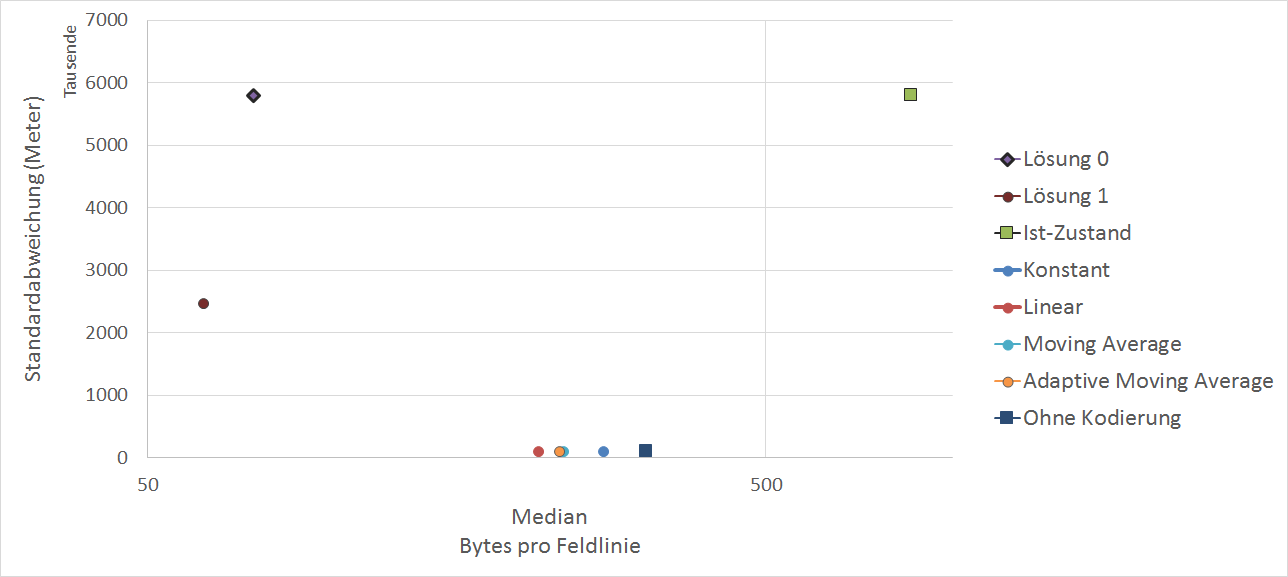
\includegraphics[width=1\textwidth,keepaspectratio]{./pictures/resultate/loesung2/variante0/resultate_byte.png}
	\caption{Artefakte der abschliessenden Variante. Links ohne Glättung, rechts mit Glättung}
	\label{resultate:loesung2:simple:resultate_byte}
\end{figure}
Der Linare Prediktor kann eine Feldinie mit etwa $214$ Bytes darstellen, was eine Kompressionsrate von $4$ ergibt. Auf kosten der Qualität wird versucht eine bessere kompressionsrate zu erreichen.

\subsubsection{Variante: Adaptiven Subsampling}
Gute Möglichkeit viele informationen zu verlieren.
Figure
schwieriger zu quantisieren, da weniger Stetig. Kurven der PCA. Möglichkeit eine Variante Prediktive kodierung für Kurven, wird aber einiges komplexer.
Einfacher wenn Kodierung für
Figure
Sphärisches Koordinatensystem.Einfacher abzuspeichern
POW
Aber Ebenfalls schwer vorherzusagen

\subsubsection{Wavelet Prediktive Kodierung}
beschrieben im Abschnitt \ref{konzept:prediktiv}
figure
figure psnr-hvs-m
